\documentclass[a4j,8pt]{jarticle}
%\documentclass[a4j,multicol,8pt]{jarticle}
%\documentclass[a4j,twocolumn,8pt]{jarticle}
\usepackage[top=15truemm,bottom=20truemm,left=15truemm,right=15truemm]{geometry}
\usepackage[dvipdfmx]{graphicx}
\usepackage{url}
\usepackage{here}
\usepackage{caption}
\usepackage{multicol}
\renewcommand{\figurename}{Fig.}
\newcommand{\Figref}[1]{Fig~\ref{#1}}
\setlength\textfloatsep{0pt} % 本文と図の間の余白
\setlength\abovecaptionskip{1pt} % 図とキャプションの余白
\usepackage{titlesec}
\titleformat*{\section}{\large\bfseries}
% あがき
%\renewcommand{\baselinestretch}{0.75}
%\setlength\abovecaptionskip{1truemm}
%\setlength\belowcaptionskip{1truemm}
\makeatletter
%\def\section{\@startsection {section}{1}{\z@}{-2.5ex plus -1ex minus -.2ex}{2.5 ex plus .2ex}{\Large\bf}}
%\def\subsection{\@startsection {subsection}{1}{\z@}{0.5ex}{0.5 ex}{\large\bf}}
%\def\subsection{\@startsection {subsection}{1}{\z@}{-1.0ex plus -1ex minus -.1ex}{3.0 ex plus .2ex}{\Large\bf}}
%\def\subsubsection{\@startsection {subsubsection}{1}{\z@}{-2.5ex plus -1ex minus -.2ex}{.3 ex plus .2ex}{\large \bf $\spadesuit$ }}
\@dblfptop 0pt
\makeatother
%\makeatletter
%  \renewcomand{\section}{
%    \@startsection{section}{1}{\z@}
%    {0.4\Cvs}{0.1\Cvs}
%    {\nomalfont\large\headfont\raggedright}}
%\makeatother

\begin{document}

\pagestyle{empty} 
\title{\Large 
Numerical experiments of surface flows on giant planets \\
produced by forcings representing thunderstorms
%Numerical experiments of giant planet surface flows  \\
%produced by forcings representing thunderstorms
}
%\title{\Large 
%雷雲を想定した強制により生じる巨大惑星表層流の数値計算
%}

\author{\large Ryoma Suzuki (Planetary and Space Group)}
%\author{\large 鈴木 綾馬 (惑星宇宙グループ)}
\date{}
\maketitle
%\begin{multicols}{2}
%\vspace{-0.2zh}
\begin{center}
\bf \large Abstract
%\section*{abstract}
\end{center}
%\section{はじめに}
%\vspace{-0.8zh}
%
%%%
It is known that the surfaces of giant planets 
have the banded structures consisting of 
equatorial jets with wide latitudinal widths
and mid-latitudinal jets with narrow latitudinal widths, 
and the vortex structures in the polar regions.
Large-scale structures such as banded structures 
and polar vortices can be formed from small-scale turbulence 
due to the inverse cascade effect(e.g. Showman et al., 2009).
Thunderstorms are considered to be a candidate for 
causing such small-scale turbulence (e.g. Ingersoll et al., 2000).

Showman (2007) and Brueshaber et al. (2019) performed calculations 
in the framework of the shallow water system with 
the mass forcing representing thunderstorms.
Showman (2007) showed the formation of the banded structures
with restricting the computational domain to the latitude range of
$0^\circ - 70^\circ$ and the longitude range of $0^\circ - 120^\circ$.
Brueshaber et al. (2019) found the polar vortex structures were formed
in the computational domain from latitude 60 degrees to high latitude.
In addition, their results showed that the number and size of polar vortices, 
and the sign of vorticity significantly depend on the value of 
Burger number ($Bu \equiv (L_d/a)^2$, $L_d$ : deformation radius, $a$ : planetary radius).
However, computational domains used by previous studies 
are restricted to a part of the sphere.
In the case of regional model, the structure of jets and vortices 
may change due to momentum transport from
regions outside the restricted computational domain.

The purpose of this study is to perform global calculations and 
to investigate whether the jet and polar vortex structures
can be formed by the mass forcing representing thunderstorms.
Then, these structures are compared with the results obtained 
in previous studies to validate the domain calculations.
The model used in this study is the Hierarchical 
Spectral Models for GFD (SPMODEL; Takehiro et al. 2006, Takehiro et al. 2013).
The used equations are 1.5-layer shallow water equations 
with the mass forcing representing thunderstorms.
The experimentals are performed with changing values of the Burger number.

Standard experiment was performed with the values of 
planetary radius and rotation rate same as those of Jupiter, and $Bu = 9.72 \times 10^{-5}$.
In Standard experiment, all of mass forcing was assumed to be positive.
In the Standard experiment, the banded structure and the polar vortex structure were formed.
It was also found that the structures remained almost unchanged 
even if the positive / negative ratio of the mass forcing and the spatial size were varied.
The characteristics of the polar vortex changed according to the value of Burger number :
when the Burger number is small, small multiple vortices (Radii of $\sim$ 5 degrees) are formed, as observed Jupiter,
and as the Burger number increases, a single cyclonic vortex (Radii of 10-20 degrees) is formed, 
as observed on Saturn, Uranus, and Neptune (Fig.1).
These results are consistent with the results of Showman (2007) and Brueshaber et al. (2019).
Moreover, the results using the same parameters as in Showman (2007) show 
that the zonal wind speed of the equatorial jet is about 10 times larger than their results.
The result possibly suggests that the existences of polar regions and/or opposite hemisphere,
which was not considered in Showman (2007), affect the strength of the jet.
%
\begin{figure*}[b]
  \begin{center}
  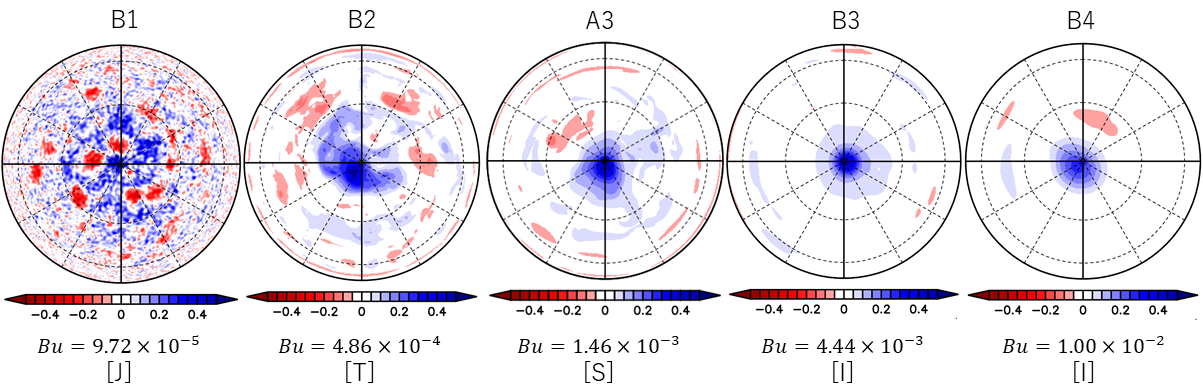
\includegraphics[width=10cm]{./fig/case1_nonqv_a.png}
  \caption{ \footnotesize Nondimensional potential vorticity : $Q_e^*$ for various values of Burger number.}
\captionsetup{labelformat=empty,labelsep=none}
\caption{\footnotesize Positive (Negative) values of $Q_e^*$ are cyclonic (anticyclonic).}
  \label{case1:nonqv_a}
  \end{center}
\end{figure*}
%
%
\end{document}
